% Template for ICASSP-2021 paper; to be used with:
%          spconf.sty  - ICASSP/ICIP LaTeX style file, and
%          IEEEbib.bst - IEEE bibliography style file.
% --------------------------------------------------------------------------
\documentclass{article}
\usepackage{spconf,amsmath,amssymb,amsfonts}
\usepackage{cite}
\usepackage{tabularray}
\usepackage{graphicx}
% Example definitions.
% --------------------


% Title.
% ------
\usepackage{booktabs}
\usepackage{multirow}
\usepackage{subcaption}
\DeclareMathOperator*{\argmin}{arg\,min}

%\title{Towards acoustic segmentation explanation through non-negative matrix factorization}
\title{An explainable proxy model for multilabel acoustic segmentation}
%
% Single address.
% ---------------
%
% For example:
% ------------
%\address{School\\
%	Department\\
%	Address}
%
% Two addresses (uncomment and modify for two-address case).
% ----------------------------------------------------------
% \twoauthors
 % {M. Lebourdais,\\\textit{M. Tahon, A. Laurent, S. Meignier, A. Larcher}}
	% {Le Mans Université\\
	% LIUM}
 % {T. Mariotte,\\\textit{S. Montrésor, J-H. Thomas}}
	% {Le Mans Université\\
	% LAUM}

\name{Théo Mariotte, Antonio Almudevar, Marie Tahon}

\address{$^{\dagger}$LIUM, $^{\diamond}$LAUM UMR 6613 IA-GS, Le Mans Université\\
theo.mariotte@univ-lemans.fr
}

\begin{document}
\ninept

\maketitle
%
\begin{abstract}
\end{abstract}
%
\begin{keywords}
acoustic segmentation, explainability, non-negative matrix factorization
\end{keywords}
%

\section{Introduction}

In the last few years, multimedia data collection has shown a noticeable increase.
Large-scale multimedia data collection requires storing and indexing massive databases.
Annotating this data is a tiresome task and can hardly be conducted manually.
Hence, the need for automatic approaches is growing.
The prevailing methodologies in the present context are primarily centered around neural networks.
However, the relationship between the input data and the decision is mostly untraceable.
The lack of knowledge in the decision-making process can be an issue in some contexts (e.g. forensic, broadcast news automatic labeling...). 
This paper focuses on automatic audio segmentation, i.e. the detection of homogeneous segments containing speech (SAD), music (MD), noise (ND), and overlapped speech (OSD) with a unified model.
This task is initially performed by a black-box neural model. 
We propose a proxy explainable model which is trained to fit the original model distribution while showing noticeable explanation capacities. 

%Historically, audio signal segmentation is performed using statistical models.
Early studies on speech \cite{sohn1999statistical}, overlapped speech \cite{charlet_impact_2013}, and music \cite{lavner2009decision} segmentation are focused on the statistical modeling of manually extracted acoustic features.
Currently, the segmentation is performed with neural networks and supervised learning.
Most approaches consist of the classification of acoustic features at the frame level.
Each task was first solved separately as binary frame classification tasks.
SAD \cite{lavechin2019end}, OSD \cite{bullock_overlap-aware_2020,lebourdais22_interspeech}, MD \cite{jang2019music,de2019exploring}.
Several approaches have also been proposed to solve multiple tasks simultaneously.
For example, in \cite{gimeno2020multiclass}, authors propose to segment speech, music, and noise with a single multiclass model.
A few works also report joint SAD and OSD \cite{jung21_interspeech,bredin21_interspeech,lebourdais2023joint}.
In this paper, SAD, OSD, MD, and ND are simultaneously solved as a multilabel frame-classification task.

The proposed approach aims to train an explainable proxy model from the black-box pre-trained segmentation system.
While many works have been conducted in explaining neural networks \cite{}, the literature is limited in the audio domain.
The first intents are focused on saliency map extraction to reveal what information is used in the output \cite{}.
Recently, a few explainable models have been developed like APNet \cite{zinemanas2021interpretable}, which extends the prototypical network to the audio domain.
The proposed architecture is mainly inspired by \cite{parekh2023tackling}.
The authors propose to explain an audio classification model by a proxy model which is optimized to classify audio scenes while reconstructing the audio with the non-negative matrix factorization framework \cite{lee2000algorithms}.
This model can be used both as post-hoc and by design explainability.

In this paper, we propose to train an explainable proxy model from a pre-trained multilabel segmentation model (designated as the teacher).
This model inputs Wavlm pre-trained features and outputs the pseudo probability of each class.
Two types of proxy models are investigated.
The former inputs a spectrogram as features and the latter uses the teacher's Wavlm outputs.
The proxy models are inspired by \cite{parekh2023tackling}.
We demonstrate that proxy models provide similar or even better performance as the original model while being smaller and explainable.
We show that the relevant information for classification can be mapped to the spectral domain.
The relevance is confirmed by a confidence measure.
To the best of our knowledge, this is the first intent to design an explainable neural segmentation model.  

This paper is arranged as follows: sect. \ref{sect:models} presents the structure of the system along with the proxy model training strategy.
Sect. \ref{sect:protocol} introduces the experimental protocol and sect. \ref{sect:perf} the segmentation results. 
Sect. \ref{sect:explain} demonstrates the explainability capacities of the proposed system.










\section{NMF-based explainable model}

\begin{figure}[ht]
    \centering
    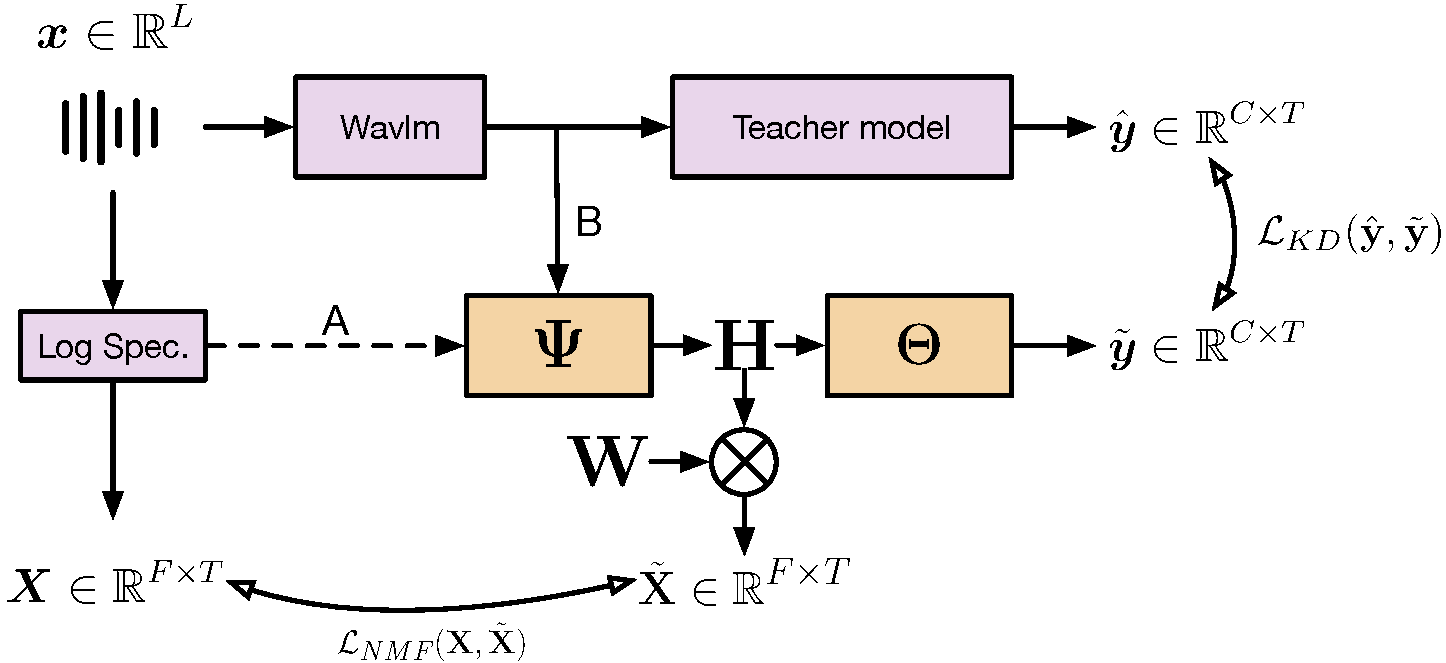
\includegraphics[width=\linewidth]{figs/nmf_model_icassp.pdf}
    \caption{Diagram of the proposed architecture for NMF-based multilabel segmentation explanation.}
    \label{fig:enter-label}
\end{figure}

\subsection{Multilabel segmentation formulation}

Acoustic segmentation is solved as a multilabel framewise classification task.
Let $\mathcal{S}=\{\mathbf{X}, \mathbf{y}\}$ be a training set composed of sequences of acoustic features $\mathbf{X}\in\mathbb{R}^{D\times T}$, where $D$ is the feature vector dimension and $T$ the number of frames, and aligned annotations $\mathbf{y}\in \mathbb{R}^{C\times T}$, with $C$ being the number of classes. 
Let $f:\mathbb{R}^{D\times T} \rightarrow \mathbb{R}^{C\times T}$ be a parametric function that estimates the logits for each class from the sequence of features such as $\hat{\mathbf{y}}=f(\mathbf{X})$.
The parameters of $f$ are optimized to minimize a loss function $\mathcal{L}(\hat{\mathbf{y}},\mathbf{y})$, usually cross-entropy, with an iterative algorithm.

The sequence of feature $\mathbf{X}$ is extracted from the audio signal $\mathbf{x}\in\mathbb{R}^{L}$ by an additional function $\mathbf{X}=g(\mathbf{x})$. 
$L$ denotes the number of audio samples.

\subsection{Non-negative matrix factorization}

NMF has been extensively used for audio signal processing.
This approach factorizes a given non-negative matrix $\mathbf{X}\in\mathbb{R}^{F\times T}$ into two non-negative matrices: $\mathbf{W}\in\mathbb{R}^{F\times K}$, usually denoted as \textit{dictionary}, and $\mathbf{H}\in\mathbb{R}^{K\times T}$, denoted as \textit{activations}.
$K$ represents the rank of the factorization.
Both matrices are jointly learned by solving
\begin{equation}
    \mathbf{W},\mathbf{H} = \argmin_{\mathbf{W},\mathbf{H}} \|\mathbf{X}-\mathbf{W}\mathbf{H}\|_2^2,
\end{equation}
with a two-step optimization process \cite{lee2000algorithms}.
In this work, we consider the sparse NMF implementation \cite{le2015sparse} as suggested in \cite{parekh2023tackling}.
In our segmentation proxy model, the dictionary $\mathbf{W}$ is pre-learned while the activation $\mathbf{H}$ is extracted by a neural model and referred to as an embedding.
The proxy model architecture and the way NMF is integrated is described in the following subsection.

\subsection{Proxy model framework}

In this work, the $f$ model is pre-trained with frozen weights and serves as a teacher for the proxy model.
We use a similar approach as \cite{parekh2023tackling} where the proxy model is composed of two functions.
Let $\Psi$ be a function that maps a sequence of $F$-dimension feature vectors $\mathbf{S}\in \mathbb{R}^{F\times T}$ to the embedding $\mathbf{H}\in \mathbb{R}^{K \times T}$. 
The proxy model logits $\tilde{\mathbf{y}}\in\mathbb{R}^{C\times T}$ are obtained with an additional $\Theta$ function such as $\tilde{\mathbf{y}}=\Theta(\mathbf{H})$.
The spectrogram of the input audio signal $\tilde{\mathbf{X}}$ is also reconstructed from $\mathbf{H}$ with the pre-learned $\mathbf{W}$ dictionary:
\begin{equation}
    \tilde{\mathbf{X}} = \mathbf{W}\mathbf{H}.
\end{equation}

The training objective of such a model is composed of 3 loss terms.
The first trains the proxy model to mimic the teacher's decisions.
Considering multilabel segmentation, and following the common approaches in knowledge distillation \cite{}, we use the binary Kullback-Leiber (KL) divergence between the teacher and the proxy model output distributions:
\begin{equation}
\mathcal{L}_{KD}(\hat{\mathbf{y}},\tilde{\mathbf{y}})=\frac{1}{T}\sum_{t=1}^T\sum_{c=1}^C\hat{{y}}_{t,c} \log\Big(\frac{\hat{{y}}_{t,c}}{\tilde{{y}}_{t,c}}\Big) + (1-\hat{{y}}_{t,c}) \log\Big(\frac{1-\hat{{y}}_{t,c}}{1-\tilde{{y}}_{t,c}}\Big)
\end{equation}
where $c$ is the class index and $t$ the frame index.

The second loss term constrains the $\mathbf{H}$ embedding to minimize the NMF-based spectrogram reconstruction and is implemented as the squared l2-norm between the target spectrogram $\mathbf{X}$ and the reconstruction $\tilde{\mathbf{X}}$:
\begin{equation}
    \mathcal{L}_{NMF}(\mathbf{X},\tilde{\mathbf{X}})=\|\mathbf{X}-\mathbf{W}\mathbf{H}\|_2^2.
\end{equation}

The last loss term minimizes the l1-norm of the $\mathbf{H}$ embedding to enforce it to be sparse.
Having a sparse embedding reduces the number of active components, and makes the explanation step easier ().
Finally, the global training objective is the weighted sum of the 3 terms:
\begin{equation}
    \mathcal{L} = \alpha \mathcal{L}_{KD}(\hat{\mathbf{y}},\tilde{\mathbf{y}}) + \beta \mathcal{L}_{NMF}(\mathbf{X},\tilde{\mathbf{X}}) + \gamma \|\mathbf{H}\|_1,
\end{equation}
where $(\alpha, \beta, \gamma)$ is a triplet of hyperparameters to weight each term of the loss.




\section{Experimental protocol}

\subsection{Datasets}

In the current literature, there is no audio data annotated to perform SAD, OSD, MD, and ND simultaneously.
Therefore, models are trained on several datasets to perform multilabel audio segmentation so that all the classes are represented.
The teacher is trained on 4 different datasets listed in the table \ref{tab:datasets}.
Due to the large amount of data, the teacher pre-training requires a lot of resources and a long training process to converge.
We propose to train the proxy model on a subset of the training set.
Only Albayzin and DiHard data are used for the knowledge distillation step.


\begin{table}[hb]
    \centering
    \begin{tabular}{lcccccc}
         \toprule
         & \multicolumn{2}{c}{Model} & \multicolumn{4}{c}{Annotation} \\
         \cmidrule{2-3}
         \cmidrule{4-7}
         Dataset & T & P & SAD & MD & ND & OSD \\
         \midrule
         Albayzin \cite{albayzin10,albayzin12} & \checkmark & \checkmark & \checkmark & \checkmark & \checkmark &  \\
         OpenBMAT \cite{openBMAT} & \checkmark & & & \checkmark & & \\
         ALLIES \cite{larcher:hal-03262914_short} & \checkmark & & \checkmark & & & \checkmark \\
         DiHard III \cite{ryant2021dihard} & \checkmark & \checkmark & \checkmark & & & \checkmark \\
         \bottomrule
    \end{tabular}
    \caption{Datasets used to train both teacher (T) and proxy (P) models with the available labels in each of them.}
    \label{tab:datasets}
\end{table}

\subsection{Model architectures}

The teacher model is similar to \cite{lebourdais22_interspeech} and is composed of two main parts: feature extraction and sequence modeling.
The former is performed using Large Wavlm pre-trained features \cite{chen2022wavlm}.
The obtained output is a sequence of vectors of $D=1024$ dimensions.
The latter part of the model inputs the sequence of Wavlm features and applies transformations to predict the segmentation.
A bottleneck layer of 64 channels first transforms these features.
3 TCN blocks process the output of the bottleneck layer \cite{bai_empirical_2018} composed of 5 1-d convolutional layers with exponentially increasing dilatation. 
A 1-d convolution layer processes the output of the TCN blocks to project the hidden representations to the logits space.
A sigmoid activation function is then applied to get normalized scores for each class.

As described in section \ref{}, two types of proxy models are investigated.
In the first approach, the proxy model inputs a spectrogram extracted on 64ms sliding windows with 20ms step.
It is then processed by 4 block TCN models where each block comprises 4 layers.
The bottleneck and hidden layer are composed of 128 and 256 channels respectively.
The second approach uses Wavlm features from the teacher as input.
In this case, the TCN model is smaller, with 2 blocks of 3 1-d convolution layers. 
The bottleneck and hidden layer are composed of 64 and 128 channels respectively.

\subsection{NMF pre-training}

As previously introduced, the $\mathbf{W}$ dictionary is pre-trained to map the embedding space to the spectrogram space.
Two approaches were investigated.
First, we allowed the $\mathbf{W}$ dictionary to be trained with the proxy model.
In this case, the dictionary is implemented as a linear layer with no bias.
Second, the dictionary is pre-trained with the standard NMF approach and fixed during the proxy model training.
The pre-training is performed on a subset of Aragon Radio.
We select segments between 1s and 4s representing each type of class.
In practice, the subset is built with 1200 segments with 16\% of speech and 42\% of music and noise.
For each approach, the NMF rank is fixed at $K=256$.


\subsection{Evaluation procedure}

To evaluate the segmentation performance, both teacher and proxy models are evaluated following the same protocol.
Models are evaluated on Aragon Radio, DiHard III, and Allies clean test sets.
The two first datasets follow the split proposed for the original challenges \cite{albayzin12,ryant2021dihard} while the last one is a selection of files that have been re-annotated for segmentation.

\section{Segmentation performance}


\begin{table*}[ht]
    \centering
    \begin{tabular}{lcccccccc}
        \toprule
         & \multicolumn{3}{c}{Aragon Radio} & \multicolumn{2}{c}{DiHard III} & \multicolumn{2}{c}{Allies Clean Test}\\
         \cmidrule{2-4}
         \cmidrule{5-6}
         \cmidrule{7-8}
         Model ID & SAD & ND & MD & SAD & OSD & SAD & OSD & HM\\  
         \midrule
         Teacher & \textbf{96.8} & 78.6 & \textbf{93.2} & \textbf{96.9} & 60.7 & \textbf{98.8} & 58.6\\
         \midrule
         Spectrogram  & 96.3 & 73.0 &  87.6 & 95.5 & 40.1 & 94.9 & 14.1 & 0.509 \\
         Wavlm & \textbf{96.8} & \textbf{79.5} & \textbf{93.1} & \textbf{96.9} & \textbf{61.4} & 96.2 & \textbf{67.0} & 0.801\\
         \bottomrule
    \end{tabular}
    \caption{AragonRadio performance}
    \label{tab:seg_results}
\end{table*}


\subsection{Performance of the spectrogram-based student}



\subsection{Performance of the WavLM-based student}



\section{Decision explanation}
\label{sect:explain}
This section describes the explanation extraction process to identify the relevant frequency bins for the segmentation.

\subsection{Explanation extraction}

The proxy model is built on the NMF framework.
This allows to map the $\mathbf{H}=[\mathbf{h}_1,\cdots,\mathbf{h}_t,\cdots,\mathbf{h}_T]$ embedding to the frequency domain.
Furthermore, the segmentation prediction is obtained from this embedding with the $\Theta$ linear transformation.
The first step in the explanation process is to identify the $k\in [1,\cdots, K]$ NMF components that are the most relevant for classification.
We first apply a pooling operation to the embedding by averaging it over the time dimension: $z_k = \frac{1}{T}\sum_{t=1}^T \mathbf{h}_t$.
To identify the relevant components to detect the class $c$, we define a relevance vector $\mathbf{r}_c=[r_{1,c}, \cdots, r_{k,c}, \cdots r_{K,c}]$ in which each element is computed as:
\begin{equation}
    r_{k,c} = z_k \times \theta_{k,c},
    \label{eq:relevance_vector}
\end{equation}
where $\theta_{k}$ is the $k$-th weight of the linear layer associated to class $c$.

The most relevant components are selected by applying a threshold $\tau$ to \eqref{eq:relevance_vector}. 
A filtered relevance vector $\mathbf{R}_{c,\tau}$ is obtained, in which the $k$-th element is defined as:
\begin{equation}
    R_{k,c,\tau} = 
    \begin{cases}
        r_{r,k} & \text{if } r_{r,k} > \tau \\
        0       & \text{otherwise}. \\
    \end{cases}
\end{equation}

\subsection{Segment-level explanation}

The filtered relevance vector $\mathbf{R}_{c,\tau}$ belongs to the same space as the $\mathbf{H}$ embedding.
Hence, it can be projected to the frequency domain by the following NMF linear transformation:
\begin{equation}
    \mathbf{X}_{c,\tau} = \mathbf{W}\mathbf{R}_{c,\tau},
    \label{eq:rel_proj_freq}
\end{equation}
where $\mathbf{X}_{c,\tau}\in\mathbb{R}^{K}$ is the projection of the relevant components in the frequency domain given $c$ and $\tau$.
This representation highlights the relevant frequency bin to detect a given class.

After identifying the relevant components, it is necessary to measure the confidence in the model decision.
The confidence measure is obtained by only keeping the relevant components in the $\mathbf{H}$ embedding and forwarding this filtered embedding $\mathbf{H}_{c,\tau}$ through the $\Theta$ layer such that $\tilde{\mathbf{y}}_{c,\tau}=\Theta(\mathbf{H}_{c,\tau})$.
Thus, the frequency-domain explanation $\mathbf{X}_{c,\tau}$ can be compared to the model output for a given threshold $\tau$.

\begin{figure}[ht]
    \centering
    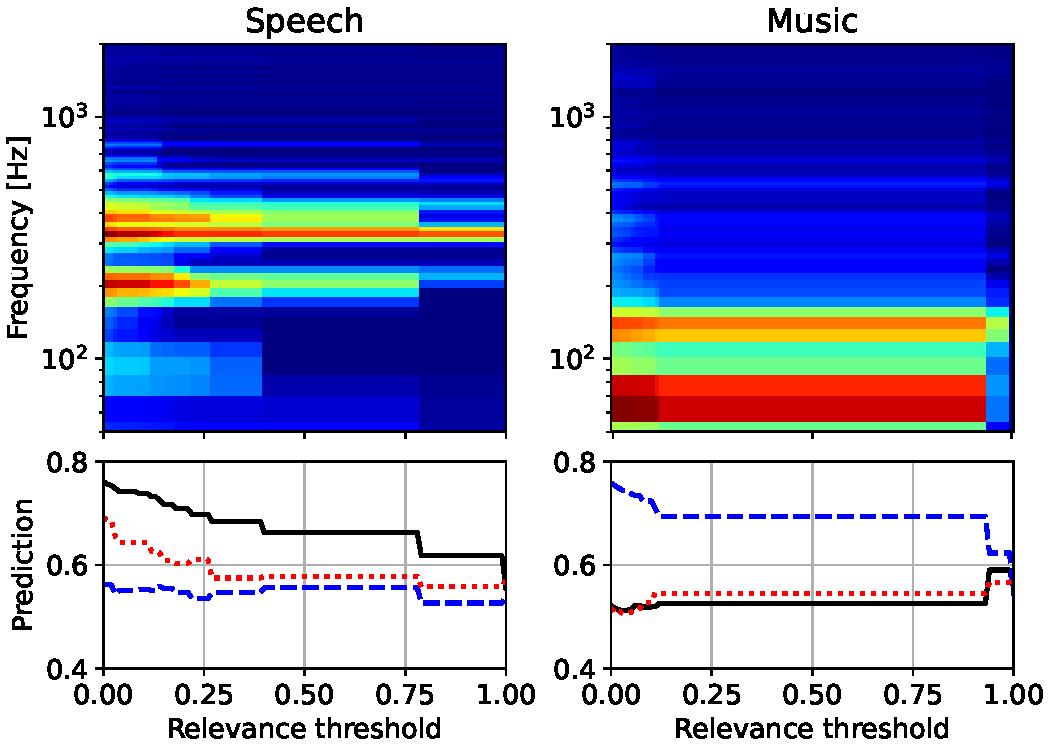
\includegraphics[width=\linewidth]{figs/icassp_rkc.pdf}
    \caption{(Top) relevant for speech and music segmentation according to the relevance threshold $\tau$. (Bottom) Model prediction for (\textbf{--}) speech, (\textbf{\textcolor{blue}{-~-}}) music, and (\textcolor{red}{$\boldsymbol{\cdots}$}) overlapped speech with each selected components.}
    \label{fig:seg_explain}
\end{figure}

Figure \ref{fig:seg_explain} shows the relevant components projected in the frequency domain with the equation \eqref{eq:rel_proj_freq} for two types of segments: speech and music.
The relevant components are presented as a function of the relevance threshold.
The model prediction obtained from the selected components is also presented.

The figure shows that the relevant components for speech are located between 100Hz and 1kHz. 
The model shows a high prediction until $\tau=0.75$. 
This allows to identify of the most relevant components for speech classification e.g., the component around $f=$200Hz.
The overlap prediction is also affected by these components.
This can be explained by the presence of common relevant frequency bins between SAD and OSD (Fig. \ref{fig:global_exp}).
However, the music prediction is similar for each $\tau$, demonstrating that the identified frequency bins are not used for MD.

In the case of MD, the relevant frequency bins are located between 50Hz and 200Hz.
The components located in the band [60,80]Hz are highly relevant for music detection.
When those are removed ($\tau$=0.9), the music prediction drops.
SAD and OSD prediction remain similar for each $\tau$ since the frequency bins are different between music and these classes.

The quality of the reconstruction limits the explanation extraction in the frequency domain.
In the case of the Wavlm-based proxy model, the reconstruction is of low quality in high frequencies. 
Thus, no explanation can be extracted in this part of the spectrum.
The following section proposes to extend the relevance component identification by global analysis.

\subsection{Global explanation}

The proposed explanation is obtained at the segment level, meaning that the relevant components are identified locally.
However, there is no guarantee that the components used to detect a class $c$ in a segment are the same across an entire dataset.
Thus, we propose a global explanation, which averages the relevance vectors $\mathbf{r}_{c}$ for a set of $N$ segments $\mathcal{D}_c=\{\mathbf{x}_{1,c}, \cdots, \mathbf{x}_{n,c}, \cdots \mathbf{x}_{N,c}\}$ containing the class of interest $c$:
\begin{equation}
    \bar{\mathbf{r}}_{c} = \frac{1}{N}\sum_{\mathbf{x}_{c}\in\mathcal{D}_c} \mathbf{r}_c.
    \label{eq:avg_rel}
\end{equation}

The $\bar{\mathbf{r}}_{c}$ vector highlights the global relevant components to detect the class $c$.

\begin{figure}[htb]
    \centering
    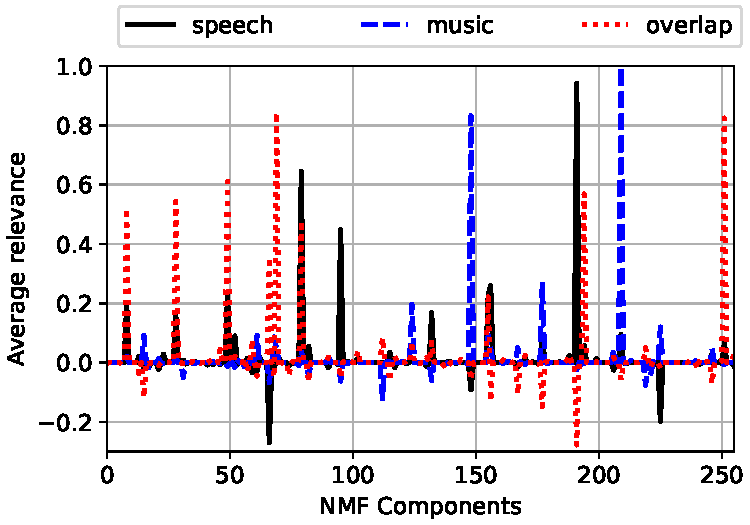
\includegraphics[width=0.8\linewidth]{figs/r_kc_acc.pdf}
    \caption{Global relevant components for speech (sp), music (mu), and overlapped speech (ov).}
    \label{fig:global_exp}
\end{figure}


To compute the average relevance of equation \eqref{eq:avg_rel}, 100 segments containing exclusively each class of interest are selected to build each subset $\mathcal{D}_c$.
To better control the OSD case, two-speaker artificial speech mixtures are generated by summing two speech segments.
The noise class is not represented since few segments contain exclusively noise.

Figure \ref{fig:global_exp} presents the average relevance $\bar{\mathbf{r}}$ for each NMF component,  computed for SAD, OSD, and MD.
It shows that some NMF components are typical for SAD and OSD.
For example, the component of index 50 is activated for both classes.
In contrast, some components discriminate between these two classes e.g., at index 70 where the speech component shows a negative relevance.
The figure also demonstrates that the NMF components related to music are different from speech and overlap ones.
This confirms the behavior observed at the segment level in figure \ref{fig:seg_explain}.

\section{Conclusions}

\newpage
\bibliographystyle{IEEEbib}
\bibliography{habi}
%\bibliography{strings}
\end{document}
